\documentclass[aspectratio=169]{beamer}

\usepackage[brazil]{babel}
\usepackage[utf8]{inputenc}
\usepackage[T1]{fontenc}
\usepackage{graphicx}
\usepackage{amsmath}
\usepackage{booktabs}
\usepackage{tikz}

\usetheme{Madrid}
\usecolortheme{default}
\setbeamertemplate{navigation symbols}{}
\setbeamertemplate{footline}[frame number]

\definecolor{ufmgblue}{RGB}{0,55,110}
\definecolor{accentred}{RGB}{210,30,30}
\definecolor{darkgray}{RGB}{55,55,55}

\setbeamercolor{structure}{fg=ufmgblue}
\setbeamercolor{title}{fg=white,bg=ufmgblue}
\setbeamercolor{frametitle}{fg=white,bg=ufmgblue}
\setbeamercolor{block title}{fg=white,bg=ufmgblue}
\setbeamercolor{block body}{bg=black!3}
\setbeamercolor{alerted text}{fg=accentred}

\graphicspath{{../report/figures/}}

\title[Planejamento de Movimento]{Planejamento de Movimento em Mapas de Ocupação}
\subtitle{A*, GVD e PRM}
\author{Pedro Antonio de Souza Campos Rodrigues}
\institute[UFMG]{Universidade Federal de Minas Gerais\\Programa de Pós-Graduação em Engenharia Elétrica}
\date{26 de junho de 2026}

\newcommand{\smalltag}[1]{\textcolor{darkgray}{\scriptsize #1}}

\begin{document}

\begin{frame}
    \titlepage
    \vspace{-0.8cm}
    \begin{center}
        
\includegraphics[height=0.7cm]{Logo_UFMG.png}
        \hspace{1.2cm}
        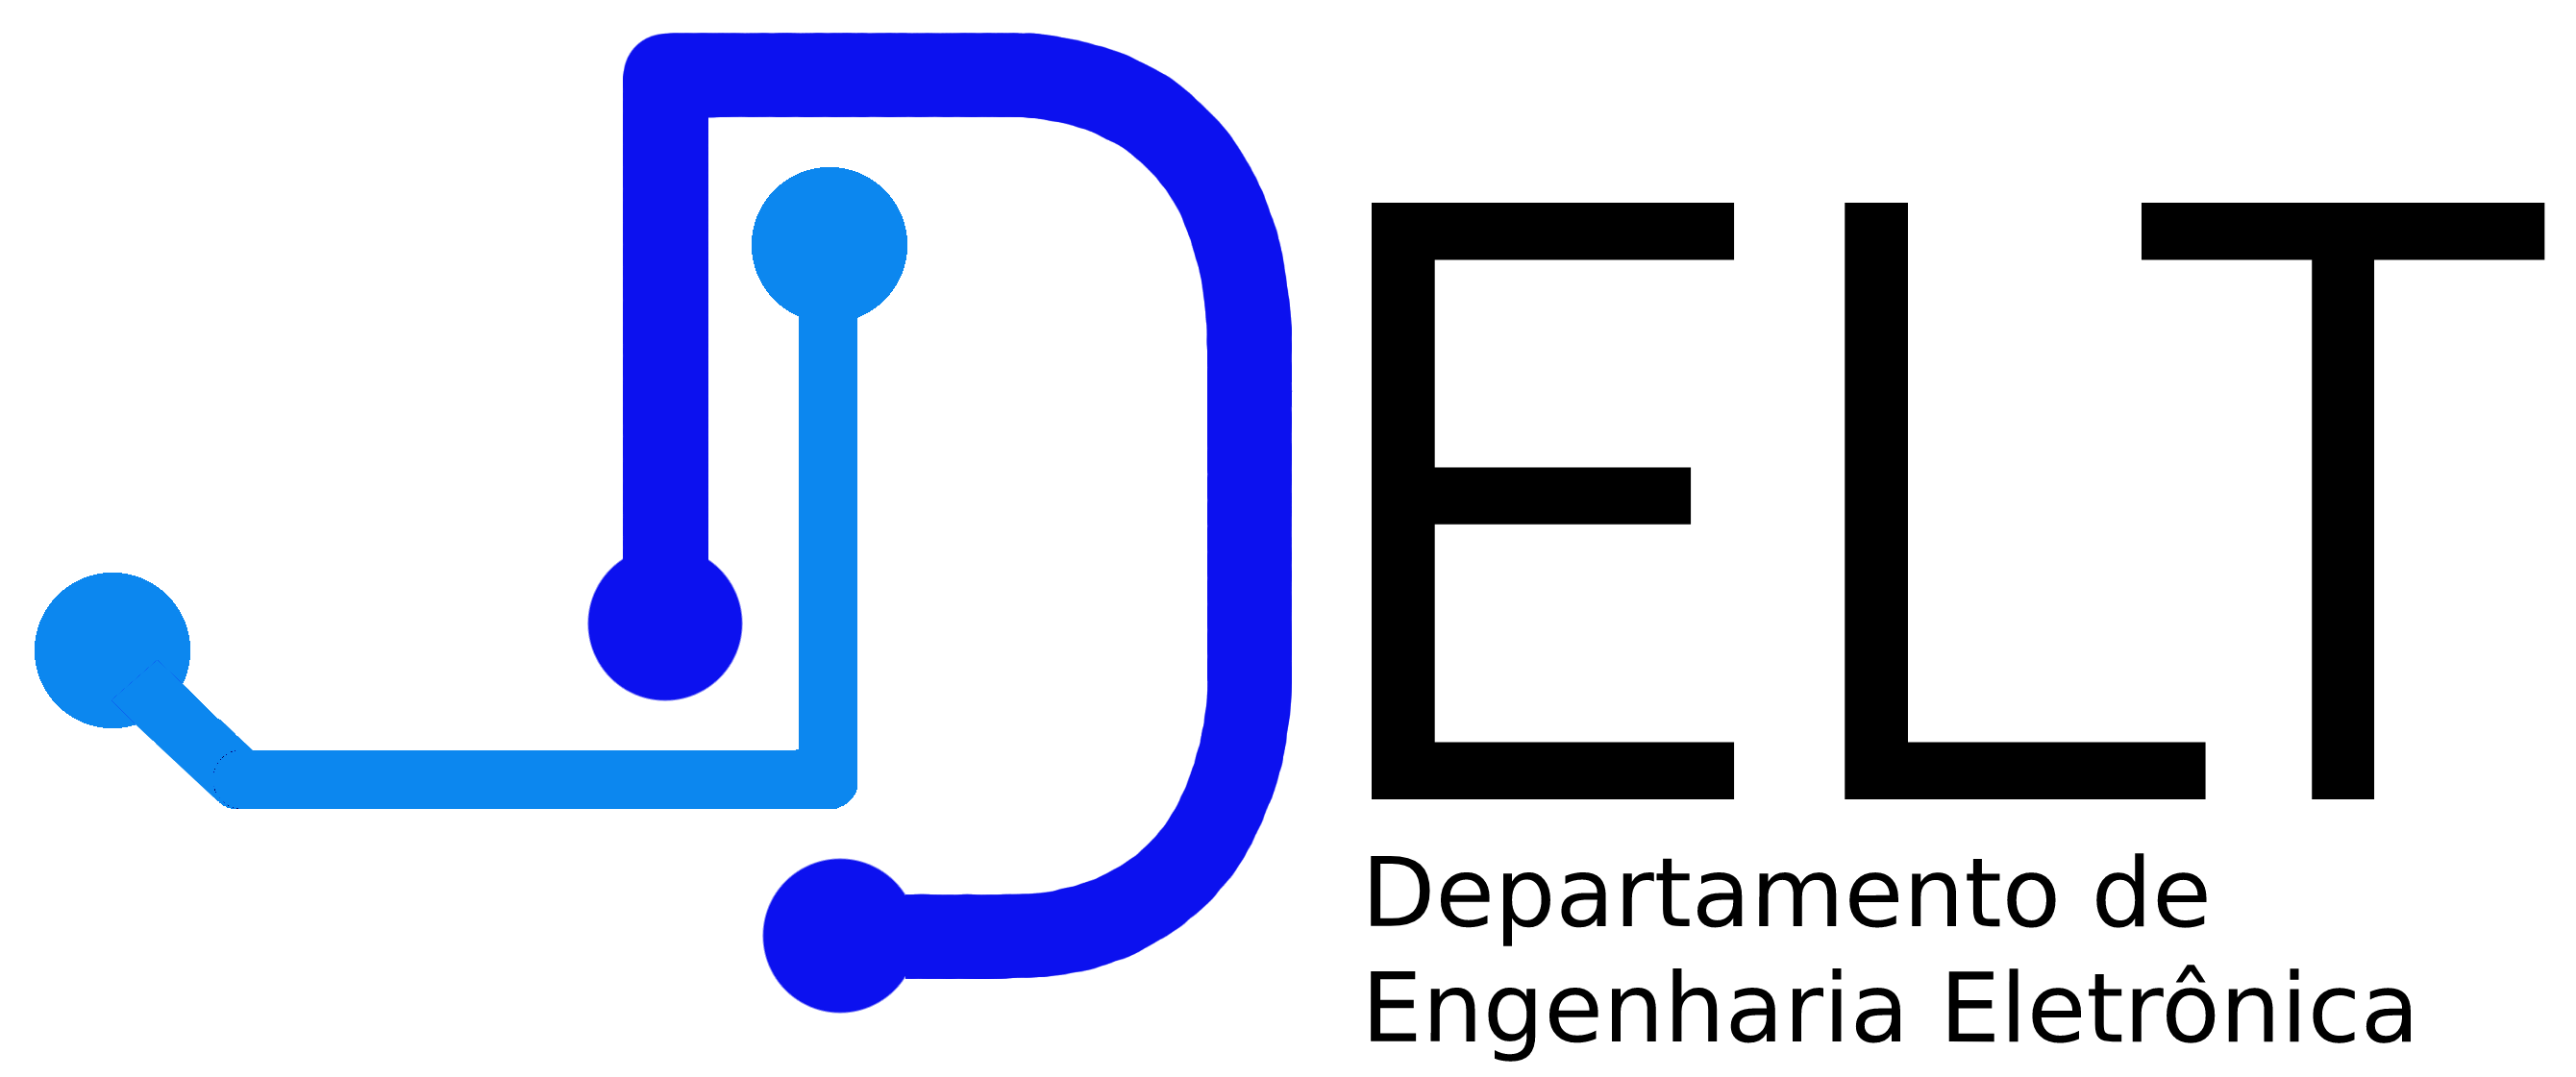
\includegraphics[height=0.7cm]{delt_logo.png}
    \end{center}
\end{frame}

\begin{frame}{Objetivo}
    \begin{block}{Problema}
        Planejar e seguir uma trajetória para um robô móvel em mapas de ocupação 2D.
    \end{block}

    \vspace{0.2cm}
    \begin{columns}[T]
        \begin{column}{0.32\textwidth}
            \textbf{A*}\\
            Busca em grade para caminhos diretos.
        \end{column}
        \begin{column}{0.32\textwidth}
            \textbf{GVD}\\
            Roadmap medial para maior afastamento dos obstáculos.
        \end{column}
        \begin{column}{0.32\textwidth}
            \textbf{PRM}\\
            Roadmap amostrado para múltiplas consultas.
        \end{column}
    \end{columns}

    \vfill
    \smalltag{Integração completa: mapa, planejamento, visualização, trajetória e controle.}
\end{frame}

\begin{frame}{Setup Utilizado}
    \begin{columns}[T]
        \begin{column}{0.38\textwidth}
            \textbf{Ambiente}
            \begin{itemize}
                \item Ubuntu 24.04.4 LTS;
                \item ROS 2 Jazzy;
                \item Gazebo Sim 8.11.0;
                \item TurtleBot3 em simulação.
            \end{itemize}

            \vspace{0.2cm}
            \textbf{Estrutura}
            \begin{itemize}
                \item RViz2 para mapa, meta e visualização;
                \item Gazebo para simular o robô;
                \item obstáculos considerados pelo mapa 2D.
            \end{itemize}
        \end{column}
        \begin{column}{0.58\textwidth}
            \centering
            \includegraphics[height=0.4\textheight,keepaspectratio]{ros2_jazzy.png}
            \hspace{0.30cm}
            \includegraphics[height=0.4\textheight,keepaspectratio]{tb3.png}

            \vspace{0.35cm}
            \includegraphics[width=0.72\linewidth]{gazebo.png}
        \end{column}
    \end{columns}
\end{frame}

\begin{frame}{Visão Geral do Sistema}
    \centering
    \begin{tikzpicture}[
        node/.style={draw, rounded corners, align=center, minimum width=2.7cm, minimum height=1.0cm, fill=black!4},
        arrow/.style={->, thick, draw=ufmgblue}
    ]
        \node[node] (map) at (0,0) {Mapa\\\texttt{/map}};
        \node[node] (planner) at (3.4,0) {Planejador\\A*, GVD ou PRM};
        \node[node] (path) at (6.8,0) {Caminho\\\texttt{Path}};
        \node[node] (traj) at (10.2,0) {Trajetória\\cúbica};
        \node[node] (ctrl) at (10.2,-2.0) {Controle\\TurtleBot3};
        \node[node] (goal) at (3.4,1.8) {Meta\\RViz2};
        \node[node] (viz) at (6.8,-2.0) {Visualização\\\texttt{MarkerArray}};

        \draw[arrow] (map) -- (planner);
        \draw[arrow] (goal) -- (planner);
        \draw[arrow] (planner) -- (path);
        \draw[arrow] (path) -- (traj);
        \draw[arrow] (traj) -- (ctrl);
        \draw[arrow] (planner) -- (viz);
    \end{tikzpicture}

    \vfill
    \smalltag{No Gazebo, o mundo foi mantido sem obstáculos físicos; as restrições vêm do mapa de ocupação.}
\end{frame}

\begin{frame}{Mapas e Inflação}
    \begin{columns}[T]
        \begin{column}{0.55\textwidth}
            \centering
            \includegraphics[width=0.31\linewidth]{map_maze.png}
            \includegraphics[width=0.31\linewidth]{map_obstacles.png}
            \includegraphics[width=0.31\linewidth]{map_random.png}

            \vspace{0.25cm}
            \includegraphics[width=0.46\linewidth]{map_inflation_original.png}
            \includegraphics[width=0.46\linewidth]{map_inflation_inflated.png}
        \end{column}
        \begin{column}{0.42\textwidth}
            \textbf{Representação binária}
            \begin{itemize}
                \item branco: região livre;
                \item preto: obstáculo.
            \end{itemize}

            \vspace{0.25cm}
            \textbf{Inflação}
            \begin{itemize}
                \item obstáculos aumentados pelo raio do robô;
                \item planejamento feito no espaço livre restante;
                \item mesma base para A*, GVD e PRM.
            \end{itemize}
        \end{column}
    \end{columns}
\end{frame}

\begin{frame}{Geração de Trajetória: Trechos}
    \begin{columns}[T]
        \begin{column}{0.48\textwidth}
            \textbf{Entrada}
            \begin{itemize}
                \item o planejador publica uma sequência de waypoints;
                \item esses pontos definem a referência geométrica;
                \item cada par consecutivo vira um trecho da trajetória.
            \end{itemize}

            \[
                \mathbf{p}_0,\mathbf{p}_1,\ldots,\mathbf{p}_N
            \]
        \end{column}
        \begin{column}{0.48\textwidth}
            \textbf{Tempo dos trechos}
            \begin{itemize}
                \item o primeiro waypoint recebe $t_0=0$;
                \item os próximos tempos são acumulados pela distância;
                \item a escala vem de \texttt{trajectory\_speed}.
            \end{itemize}

            \[
                t_{i+1}=t_i+
                \frac{\|\mathbf{p}_{i+1}-\mathbf{p}_i\|}
                {v_{\mathrm{traj}}}
            \]
        \end{column}
    \end{columns}

    \vspace{0.2cm}
    \begin{block}{Polinômio usado em cada trecho}
        \[
            \mathbf{x}_{d,i}(t)=
            \mathbf{a}_i t^3+
            \mathbf{b}_i t^2+
            \mathbf{c}_i t+
            \mathbf{d}_i,
            \qquad
            t \in [t_i,t_{i+1}]
        \]
    \end{block}
\end{frame}

\begin{frame}{Geração de Trajetória: Derivadas}
    \begin{columns}[T]
        \begin{column}{0.48\textwidth}
            \textbf{Velocidades de contorno}
            \begin{itemize}
                \item não são parâmetros escolhidos manualmente;
                \item são calculadas a partir dos waypoints vizinhos;
                \item em pontos internos, usa-se diferença centrada.
            \end{itemize}

            \[
                \mathbf{v}_i =
                \frac{\mathbf{p}_{i+1}-\mathbf{p}_{i-1}}
                {t_{i+1}-t_{i-1}}
            \]
            \smalltag{Nas extremidades, usa-se diferença progressiva ou retrógrada.}
        \end{column}
        \begin{column}{0.48\textwidth}
            \textbf{Condições de contorno}
            \begin{itemize}
                \item o trecho começa em $\mathbf{p}_i$;
                \item termina em $\mathbf{p}_{i+1}$;
                \item as derivadas nos extremos são impostas.
            \end{itemize}

            \[
                \begin{aligned}
                    \mathbf{x}_{d,i}(t_i) &= \mathbf{p}_i\\
                    \mathbf{x}_{d,i}(t_{i+1}) &= \mathbf{p}_{i+1}\\
                    \dot{\mathbf{x}}_{d,i}(t_i) &= \mathbf{v}_i\\
                    \dot{\mathbf{x}}_{d,i}(t_{i+1}) &= \mathbf{v}_{i+1}
                \end{aligned}
            \]
        \end{column}
    \end{columns}

    \vspace{0.15cm}
    \begin{center}
        \textbf{Ideia principal:} casar as derivadas entre trechos para evitar mudanças bruscas.

        \smalltag{Na execução, o controlador recebe $\mathbf{x}_d(t)$ e $\dot{\mathbf{x}}_d(t)$.}
    \end{center}
\end{frame}

\begin{frame}{Controle}
    \begin{columns}[T]
        \begin{column}{0.48\textwidth}
            \textbf{Robô diferencial}
            \begin{itemize}
                \item entradas reais: $v$ e $\omega$;
                \item não se controla $\dot{x}$ e $\dot{y}$ do centro de forma independente;
                \item solução: controlar um ponto à frente do robô.
            \end{itemize}

            \[
                \mathbf{p} =
                \begin{bmatrix}
                    x+d\cos\theta\\
                    y+d\sin\theta
                \end{bmatrix}
            \]
        \end{column}
        \begin{column}{0.48\textwidth}
            \textbf{Entrada virtual}
            \begin{itemize}
                \item definida no referencial do mundo;
                \item combina velocidade desejada e correção de erro;
                \item depois é convertida para $v$ e $\omega$.
            \end{itemize}

            \[
                \mathbf{u} =
                \dot{\mathbf{x}}_d +
                K(\mathbf{x}_d-\mathbf{p})
            \]
        \end{column}
    \end{columns}

    \vspace{0.15cm}
    \[
        \begin{bmatrix}
            v\\
            \omega
        \end{bmatrix}
        =
        \begin{bmatrix}
            \cos\theta & \sin\theta\\
            -\frac{\sin\theta}{d} & \frac{\cos\theta}{d}
        \end{bmatrix}
        \begin{bmatrix}
            u_x\\
            u_y
        \end{bmatrix}
    \]

    \smalltag{$\dot{\mathbf{x}}_d$: feedforward \quad | \quad $K(\mathbf{x}_d-\mathbf{p})$: termo proporcional}
\end{frame}

\begin{frame}{Implementação}
    \small
    A implementação foi organizada em dois pacotes ROS 2, separando os algoritmos de planejamento dos arquivos de simulação e visualização.

    \vspace{0.25cm}
    \begin{columns}[T]
        \begin{column}{0.48\textwidth}
            \textbf{\texttt{tp\_motion\_planners}}
            \begin{itemize}
                \item representação comum do mapa;
                \item A*, GVD e PRM com a mesma interface;
                \item \texttt{planner\_node} para receber mapa, pose e meta;
                \item seguidor para executar a trajetória planejada.
            \end{itemize}
        \end{column}
        \begin{column}{0.48\textwidth}
            \textbf{\texttt{tp\_simulation}}
            \begin{itemize}
                \item mapas, parâmetros e arquivos de launch;
                \item RViz2 para interação e visualização;
                \item Gazebo com mundo vazio;
                \item TurtleBot3 em simulação.
            \end{itemize}
        \end{column}
    \end{columns}
\end{frame}

\begin{frame}{A*}
	    \begin{columns}[T]
	        \begin{column}{0.45\textwidth}
	            \small
	            \textbf{Ideia}
	            \begin{itemize}
	                \item busca diretamente na grade inflada;
	                \item vizinhança 8-conectada;
	                \item fila de prioridade ordenada por custo estimado.
	            \end{itemize}

	            \vspace{-0.05cm}
	            \[
	                f(n)=g(n)+h(n)
	            \]

	            \textbf{Heurística}
	            \vspace{-0.1cm}
	            \[
	                h(n)=
	                \sqrt{(x_n-x_g)^2+(y_n-y_g)^2}
	            \]
	            \smalltag{Distância euclidiana até a meta, coerente com movimentos retos e diagonais.}

	            \vspace{0.05cm}
	            \smalltag{Característica: caminho curto e determinístico, podendo passar mais próximo dos obstáculos.}
	        \end{column}
        \begin{column}{0.52\textwidth}
            \centering
            \includegraphics[height=0.62\textheight,keepaspectratio]{resultado_astar.png}
        \end{column}
    \end{columns}
\end{frame}

\begin{frame}{GVD}
    \begin{columns}[T]
        \begin{column}{0.45\textwidth}
            \textbf{Construção}
            \begin{itemize}
                \item propagação \textit{brushfire};
                \item obstáculos e borda do mapa como fontes;
                \item frentes se encontram no eixo medial.
            \end{itemize}

            \textbf{Consulta}
            \begin{itemize}
                \item conectar início ao GVD;
                \item buscar no roadmap;
                \item sair do GVD próximo ao objetivo.
            \end{itemize}
        \end{column}
        \begin{column}{0.52\textwidth}
            \centering
            \includegraphics[width=\linewidth]{resultado_gvd.png}
        \end{column}
    \end{columns}
\end{frame}

\begin{frame}{PRM}
    \begin{columns}[T]
        \begin{column}{0.42\textwidth}
            \textbf{Construção do roadmap}
            \begin{itemize}
                \item amostrar células livres;
                \item conectar vértices próximos;
                \item validar arestas por linha reta livre.
            \end{itemize}

            \textbf{Consulta}
            \begin{itemize}
                \item acessibilidade: início $\rightarrow$ roadmap;
                \item conectividade: busca no grafo;
                \item deportabilidade: roadmap $\rightarrow$ objetivo.
            \end{itemize}
        \end{column}
        \begin{column}{0.55\textwidth}
            \centering
            \includegraphics[width=\linewidth]{resultado_prm.png}
        \end{column}
	    \end{columns}
	\end{frame}

\begin{frame}{Considerações Finais}
    \begin{itemize}
        \item Os três planejadores foram integrados ao mesmo ambiente ROS 2.
        \item O A* atende bem consultas pontuais, gerando caminhos diretos na grade.
        \item GVD e PRM funcionam como roadmaps e podem ser usados em consultas com múltiplas metas.
        \item A escolha do método depende do objetivo: caminho mais curto, maior afastamento dos obstáculos ou reutilização do planejamento.
    \end{itemize}
\end{frame}

\begin{frame}{Referências}
    \small
    \begin{itemize}
        \item Choset, H. et al. \textit{Principles of Robot Motion: Theory, Algorithms, and Implementations}. MIT Press, 2005.
        \item LaValle, S. M. \textit{Planning Algorithms}. Cambridge University Press, 2006.
        \item Notas de aula da disciplina.
    \end{itemize}
\end{frame}

\end{document}
